\documentclass[a4paper, 11pt]{article}
\usepackage{graphicx}
\begin{document}
\section{•}
Since there is no explicit/specific question or work assignment in this task, I'll simply state a few observations for the given system \textit{tipper} and then change certain traits of said system to alter those previous observations. This will hopefully show my understanding of fuzzy logic concepts and the usage of \textit{MATLAB's} corresponding designer. With these basics out of the way, I'll keep the description of task 2's new system somewhat concise and to the point.

\subsection{Selection of input and output}
Currently, there are 2 input variables (service and food) which are used to determine the value of a single output variable (tip). This is quite the logical system since service and food are probably the biggest factors for most tippers out there. To add another reasonable input variable to this setup, one could imagine a tipper who also desires a nice ambience for a generous tip. Adding \textit{ambience} results in the following system:

\begin{figure}[ht]
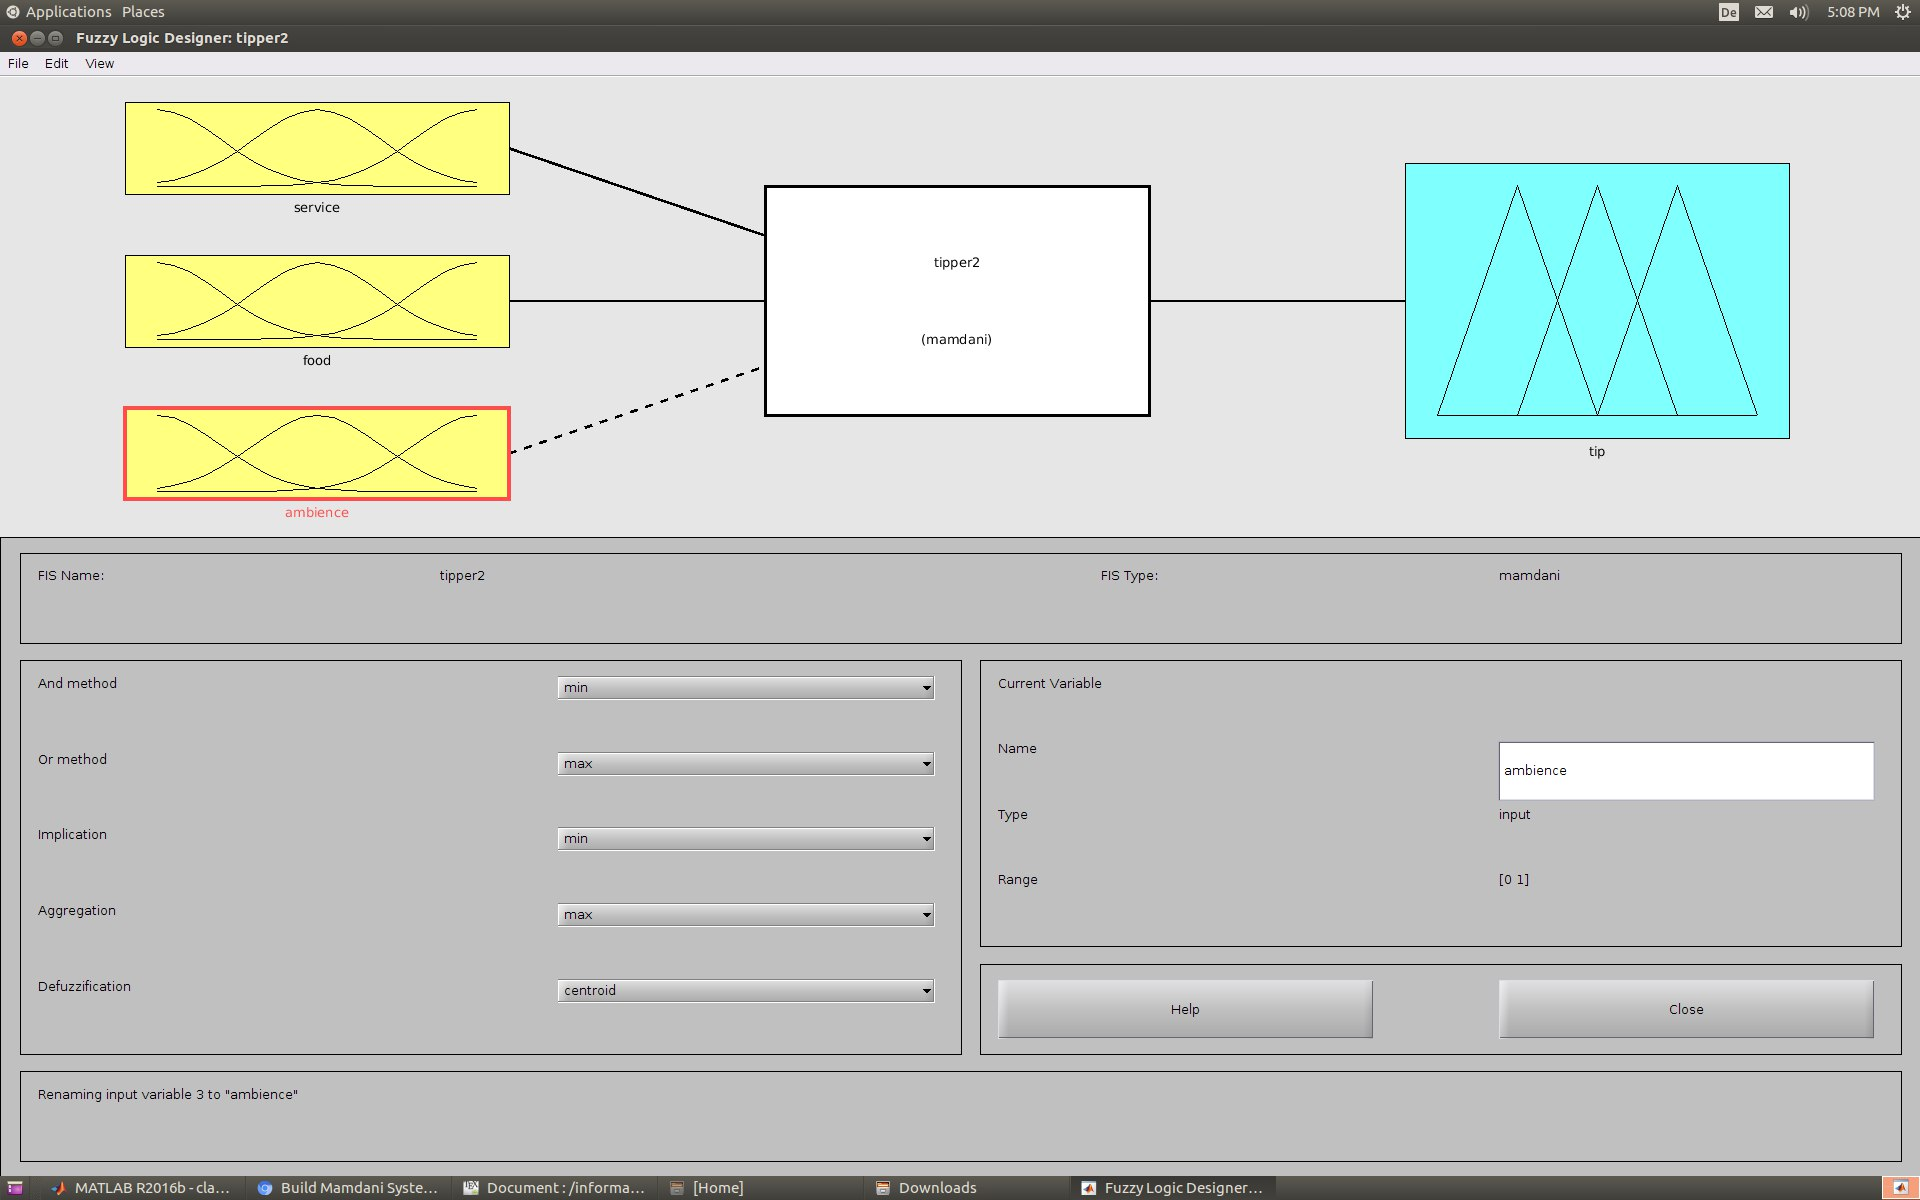
\includegraphics[scale=0.2]{1-overview.jpg}
\end{figure}
Obviously, this new variable has no impact yet, since it has no membership functions and rules associated with it.

\newpage
\subsection{Selection of different membership functions}
Membership functions by input variable:\\
\textit{Service} has three membership functions; \textit{poor}, \textit{good} and \textit{excellent} which are centered around 0, 5 and 10 respectively. Each of these are gaussian functions which makes sense for such a diverse variable.\\
\textit{Food} has two membership functions; \textit{rancid} and \textit{delicious} which hold a plateau from 0 to 1 and from 9 to 10 respectively instead of centering around a maximum value like \textit{service}. This results in two radical sides with a big whole in the middle representing a mediocre taste. This can make sense for food, because lots of people will usually only consider the taste for their foot in their tip, if it was exceptionally good or bad. Service, on the other hand, can have an influence in greater variety.\\
A sensible way of now including membership functions for our new variable \textit{ambience} could be this:

\begin{figure}[ht]
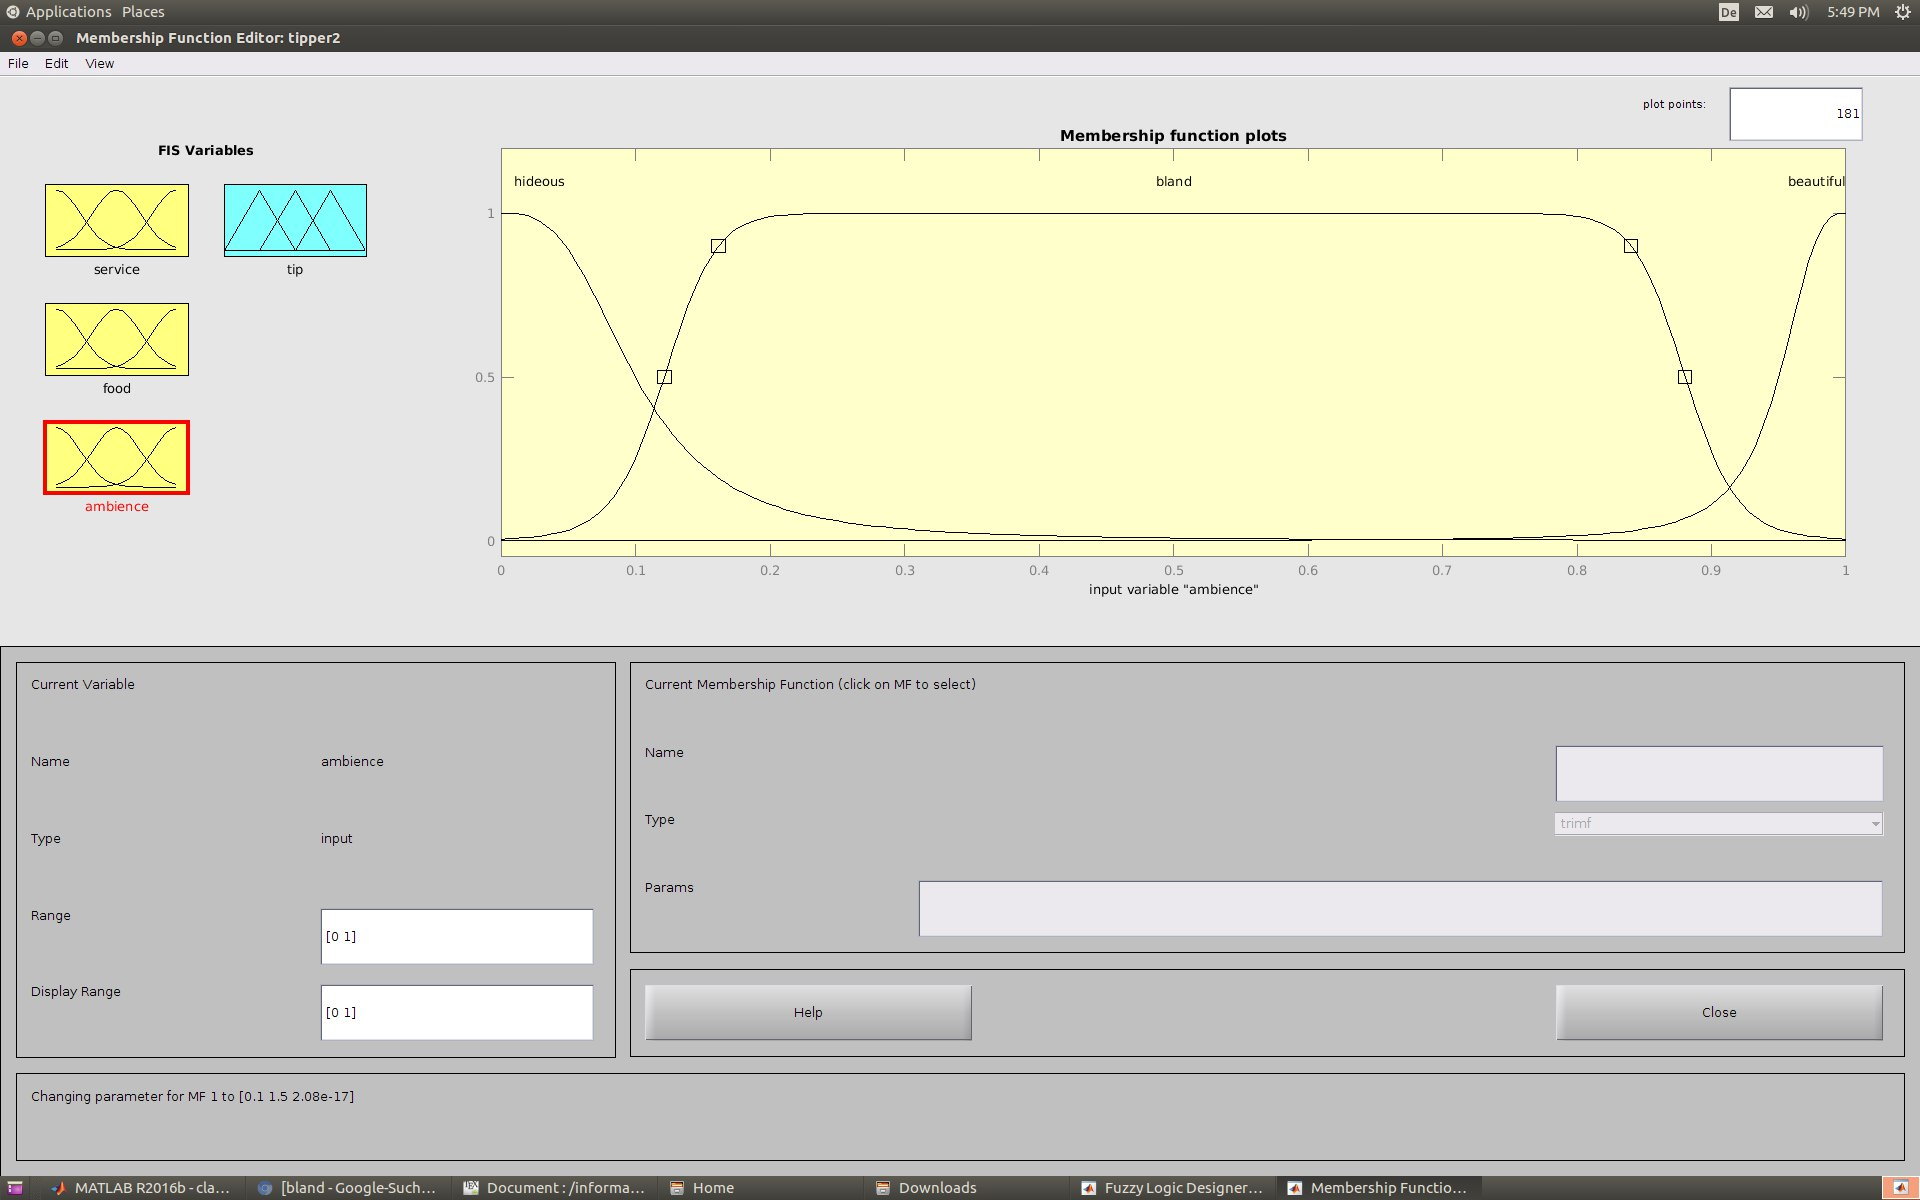
\includegraphics[scale=0.2]{ambience-mf-v2.jpg}
\end{figure}

\textit{Hideous} and \textit{beautiful} are the two extremes, while \textit{bland} serves as the mediocre area in the middle. There is a bit of an overlap between \textit{bland} and the extremes, because these descriptors aren't mutually exclusive. However, \textit{bland} does drop of to zero on both ends, because a truely hideous or beautiful restaurant really has to do something unique to invoke such an extreme impression from a tipper. Lastly, \textit{beautiful} has a steeper drop than \textit{hideous}, because the tipper in my scenario is a bit of a cynic and is more easily disappointed than impressed.

\newpage
\subsection{Creation of rules}
The basic rules for food and service are pretty simple: If any of the input variables are in the extremes of their membership functions, then the tip will also be an extreme (unless opposite extremes are met at the same time). On top of that, service has a bit more impact on the final output, because \textit{good} service will result in an \textit{average} tip, while mediocre food has no relation to the tip whatsoever.\\
Incorporating \textit{ambience} in these rules might look something like this:

\begin{figure}[ht]
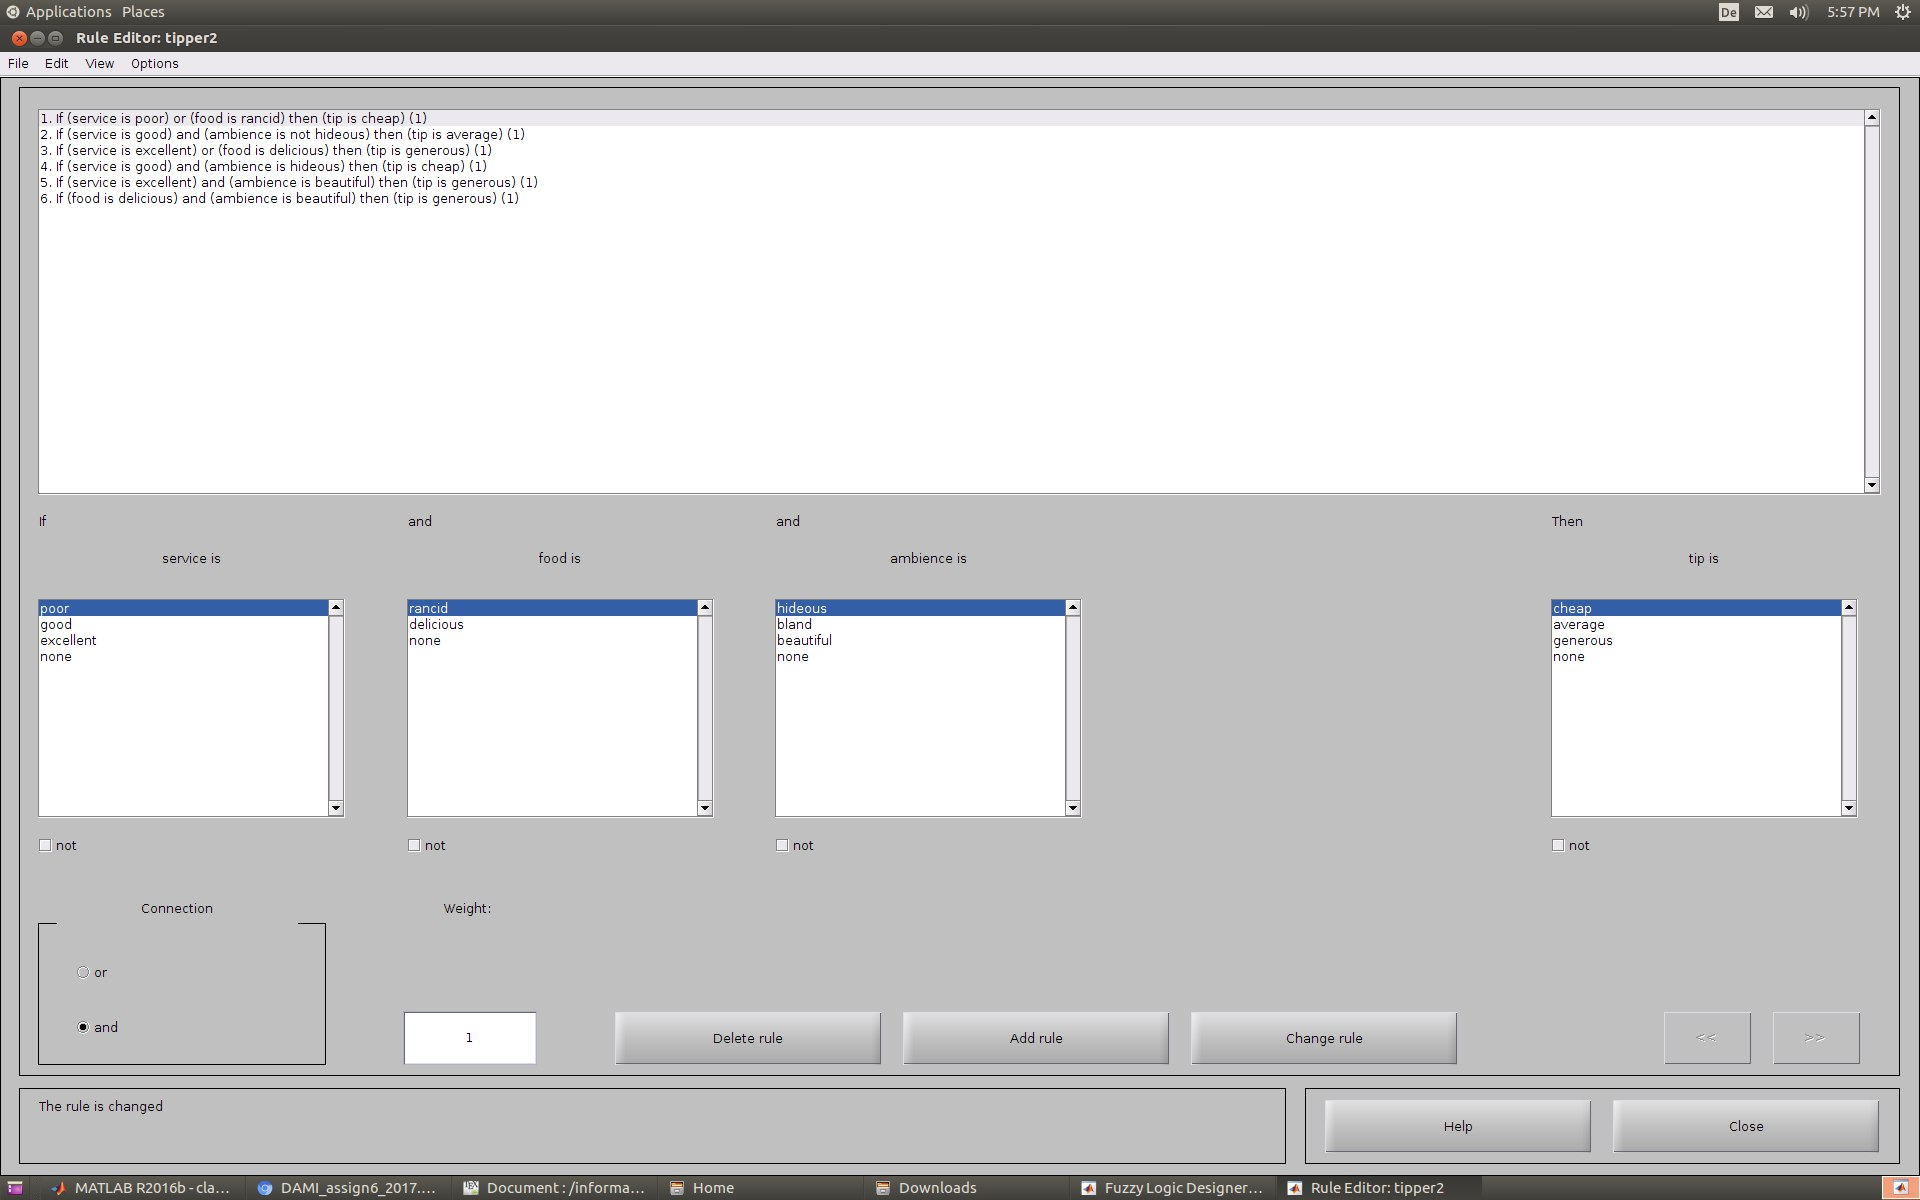
\includegraphics[scale=0.2]{ambience-rules.jpg}
\end{figure}

Here, ambience doesn't have a big influence on its own, but it has the potential to skew the tip in a certain direction, if the corresponding extreme is met.

\newpage
\subsection{Visualization}
The visualization of \textit{food} and \textit{service} is as expected: The service side has an additional bump in the middle due to \textit{good} service being mentioned in the rules. The food side is flat in the middle due it only having two extremes to consider.\\
Now to the visualizations of \textit{ambience} with the original two input variables:

\begin{figure}[ht]
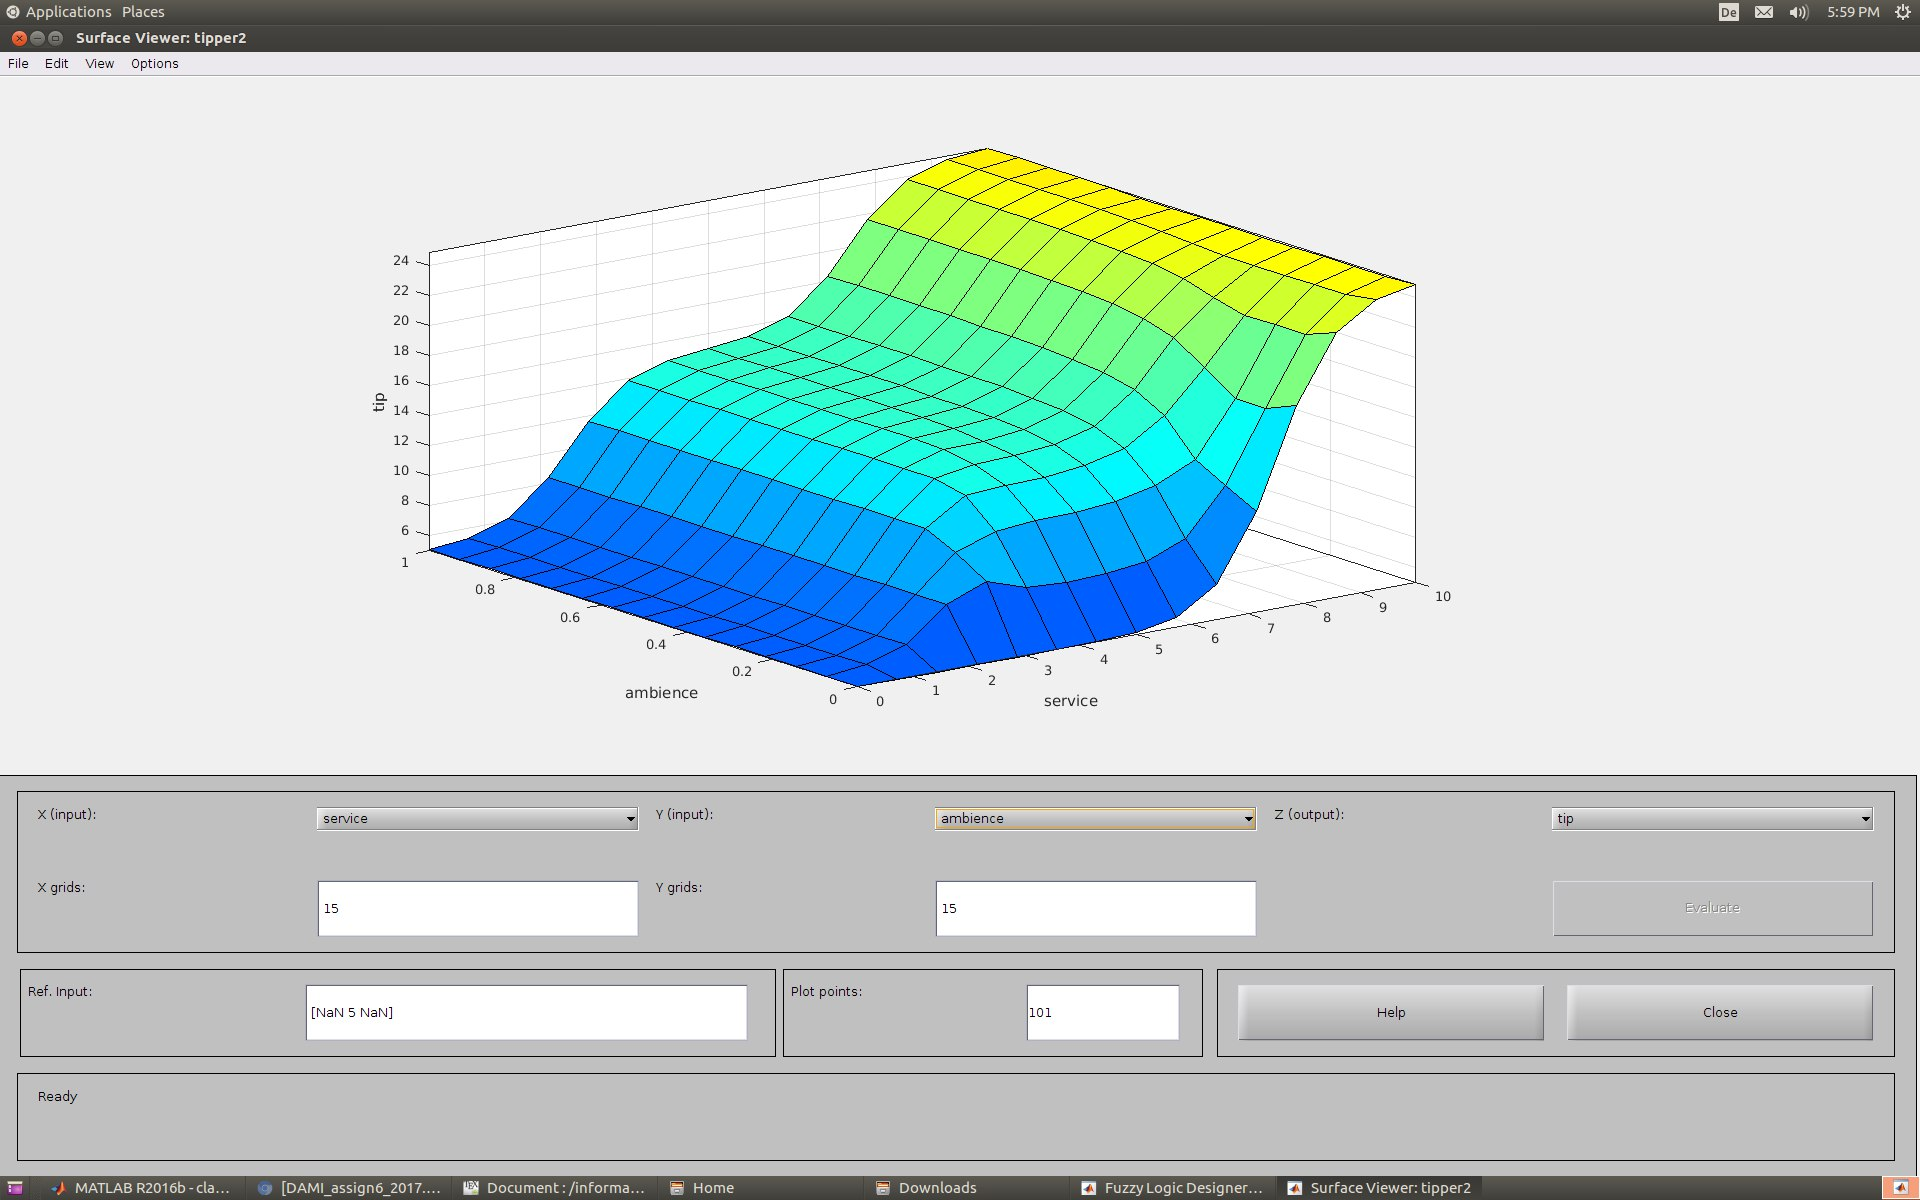
\includegraphics[scale=0.15]{ambience-surface-s.jpg}
\end{figure}

\begin{figure}[ht]
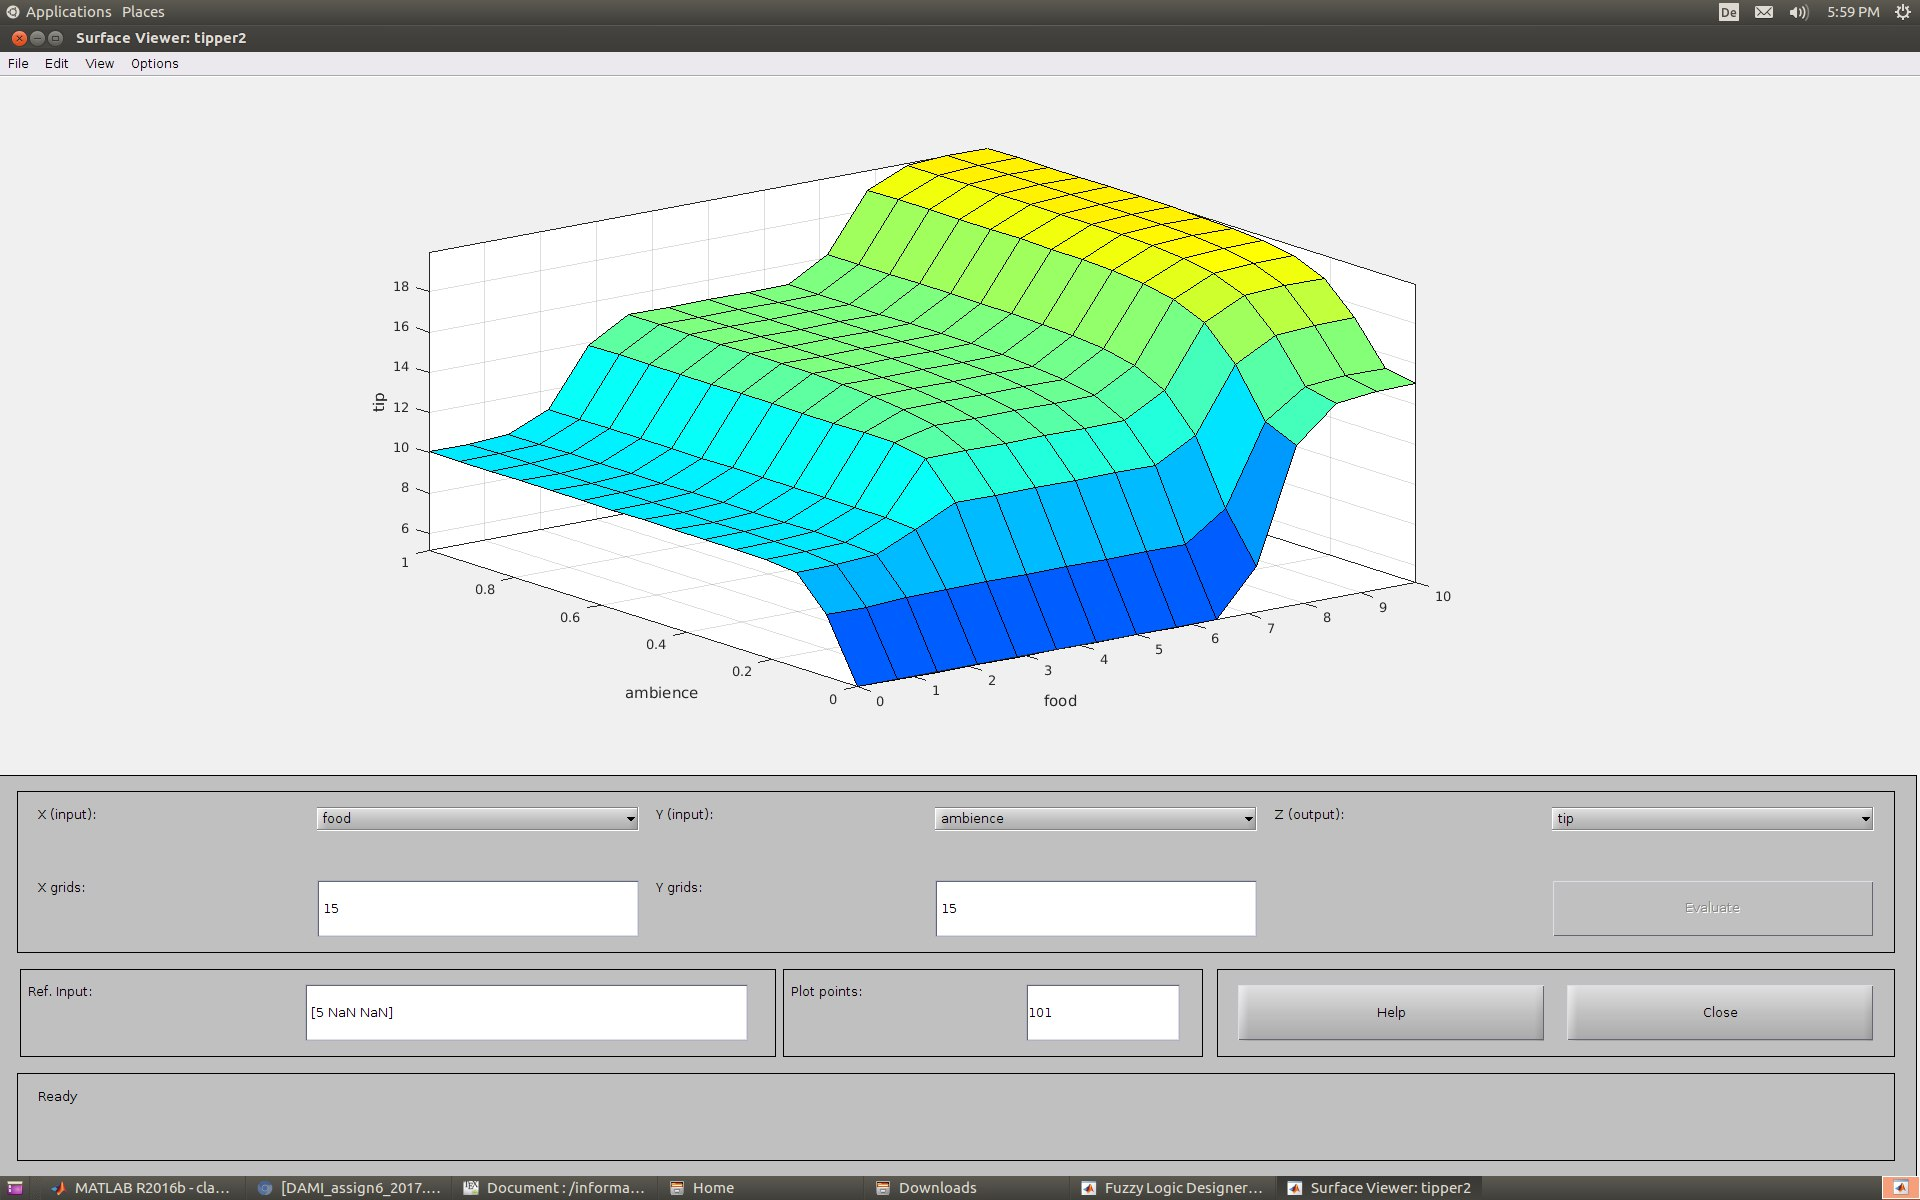
\includegraphics[scale=0.15]{ambience-surface-f.jpg}
\end{figure}

These visualizations are fairly similar except for the edges: On the lower end, great ambience cannot raise the tip, as long as service is at 0, but terrible food can still result in a 10\% tip, if the ambience isn't hideous as well.\\
The same logic applies to the upper end of the graph: Incredible service will result in the maximum tip, even if the ambience is hideous, but amazing food cannot elevate the tip over 15\% in that very same ambience.

\newpage

\section{•}
Fuzzy logic model of a videogame critic:\\
The goal of my model is to determine the audience of a given videogame. A game may be recommended to \textit{nobody}, to \textit{fans of the genre} or to \textit{everybody}. The input variables that influence this recommendation are \textit{gameplay}, \textit{story} and \textit{originality}.

\begin{figure}[ht]
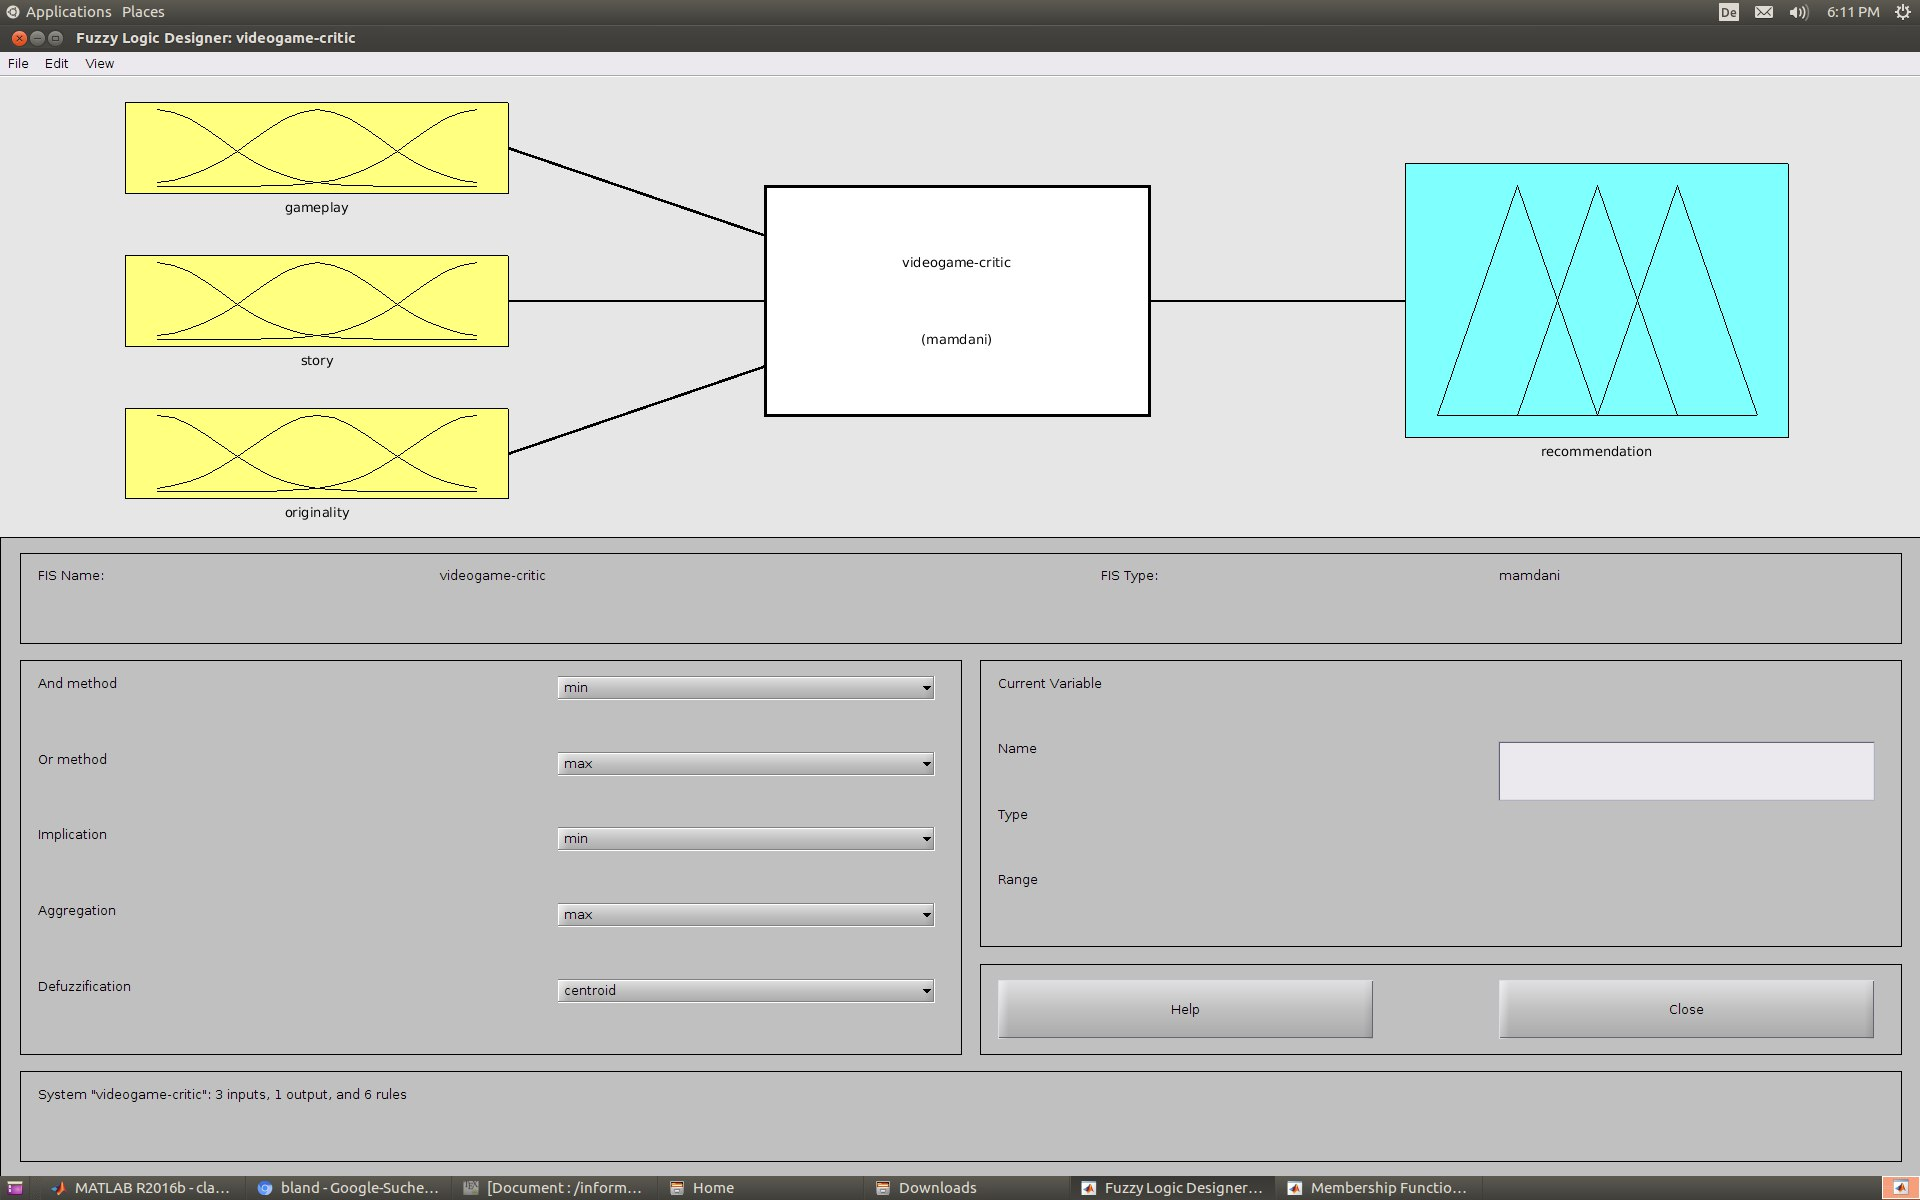
\includegraphics[scale=0.15]{vg-mf-sum.jpg}
\end{figure}

\begin{figure}[ht]
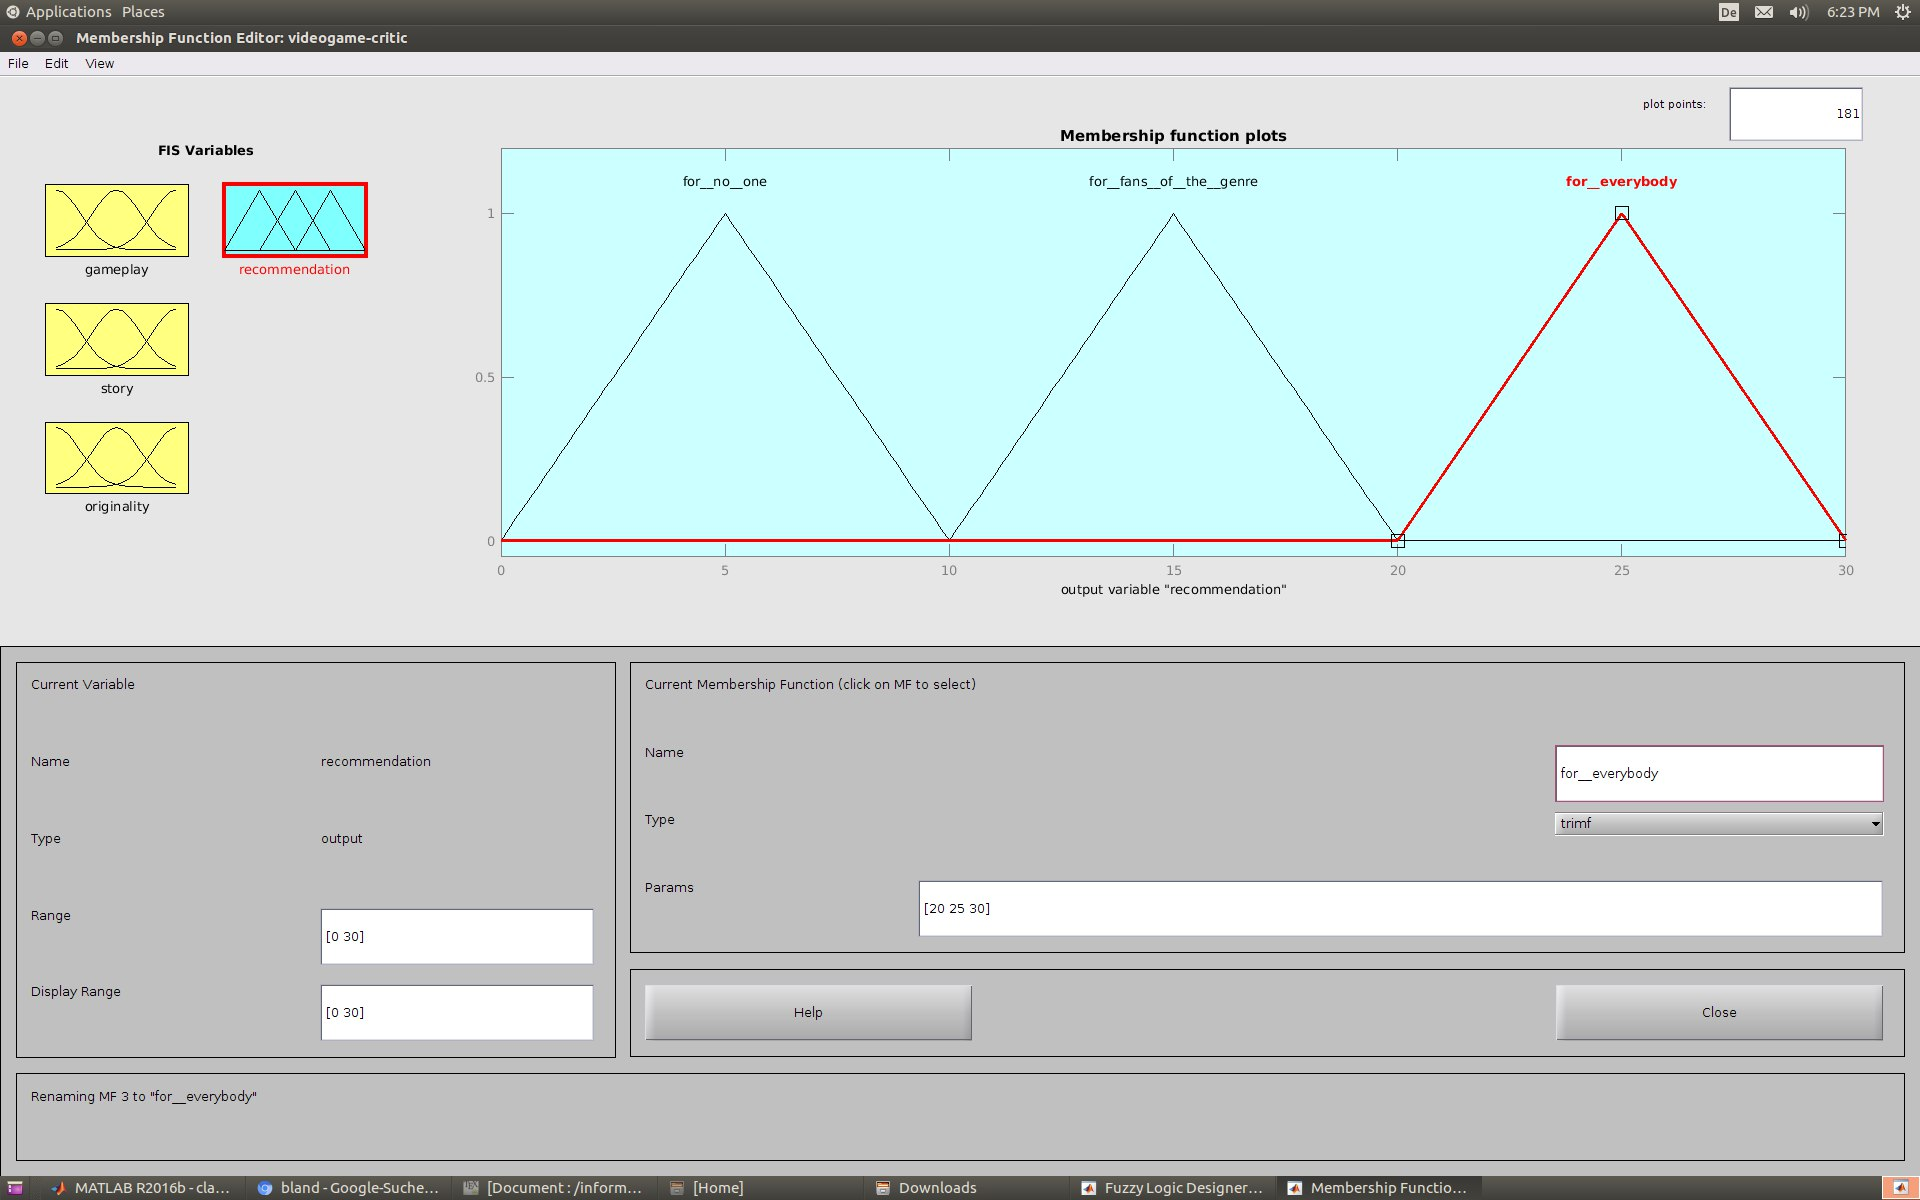
\includegraphics[scale=0.15]{vg-mf-out.jpg}
\end{figure}

\newpage

This fuzzy logic system is based on a very specific archetype of videogame critic: Someone who rates gameplay above all else. As long as a game feels good to play from beginning to end, it will probably get a good rating. And since gameplay is so important to this critic, he has a high level of expertise and can judge even the smallest properties of gameplay, resulting in a greater amount of membership functions that a game could land in. 

\begin{figure}[ht]
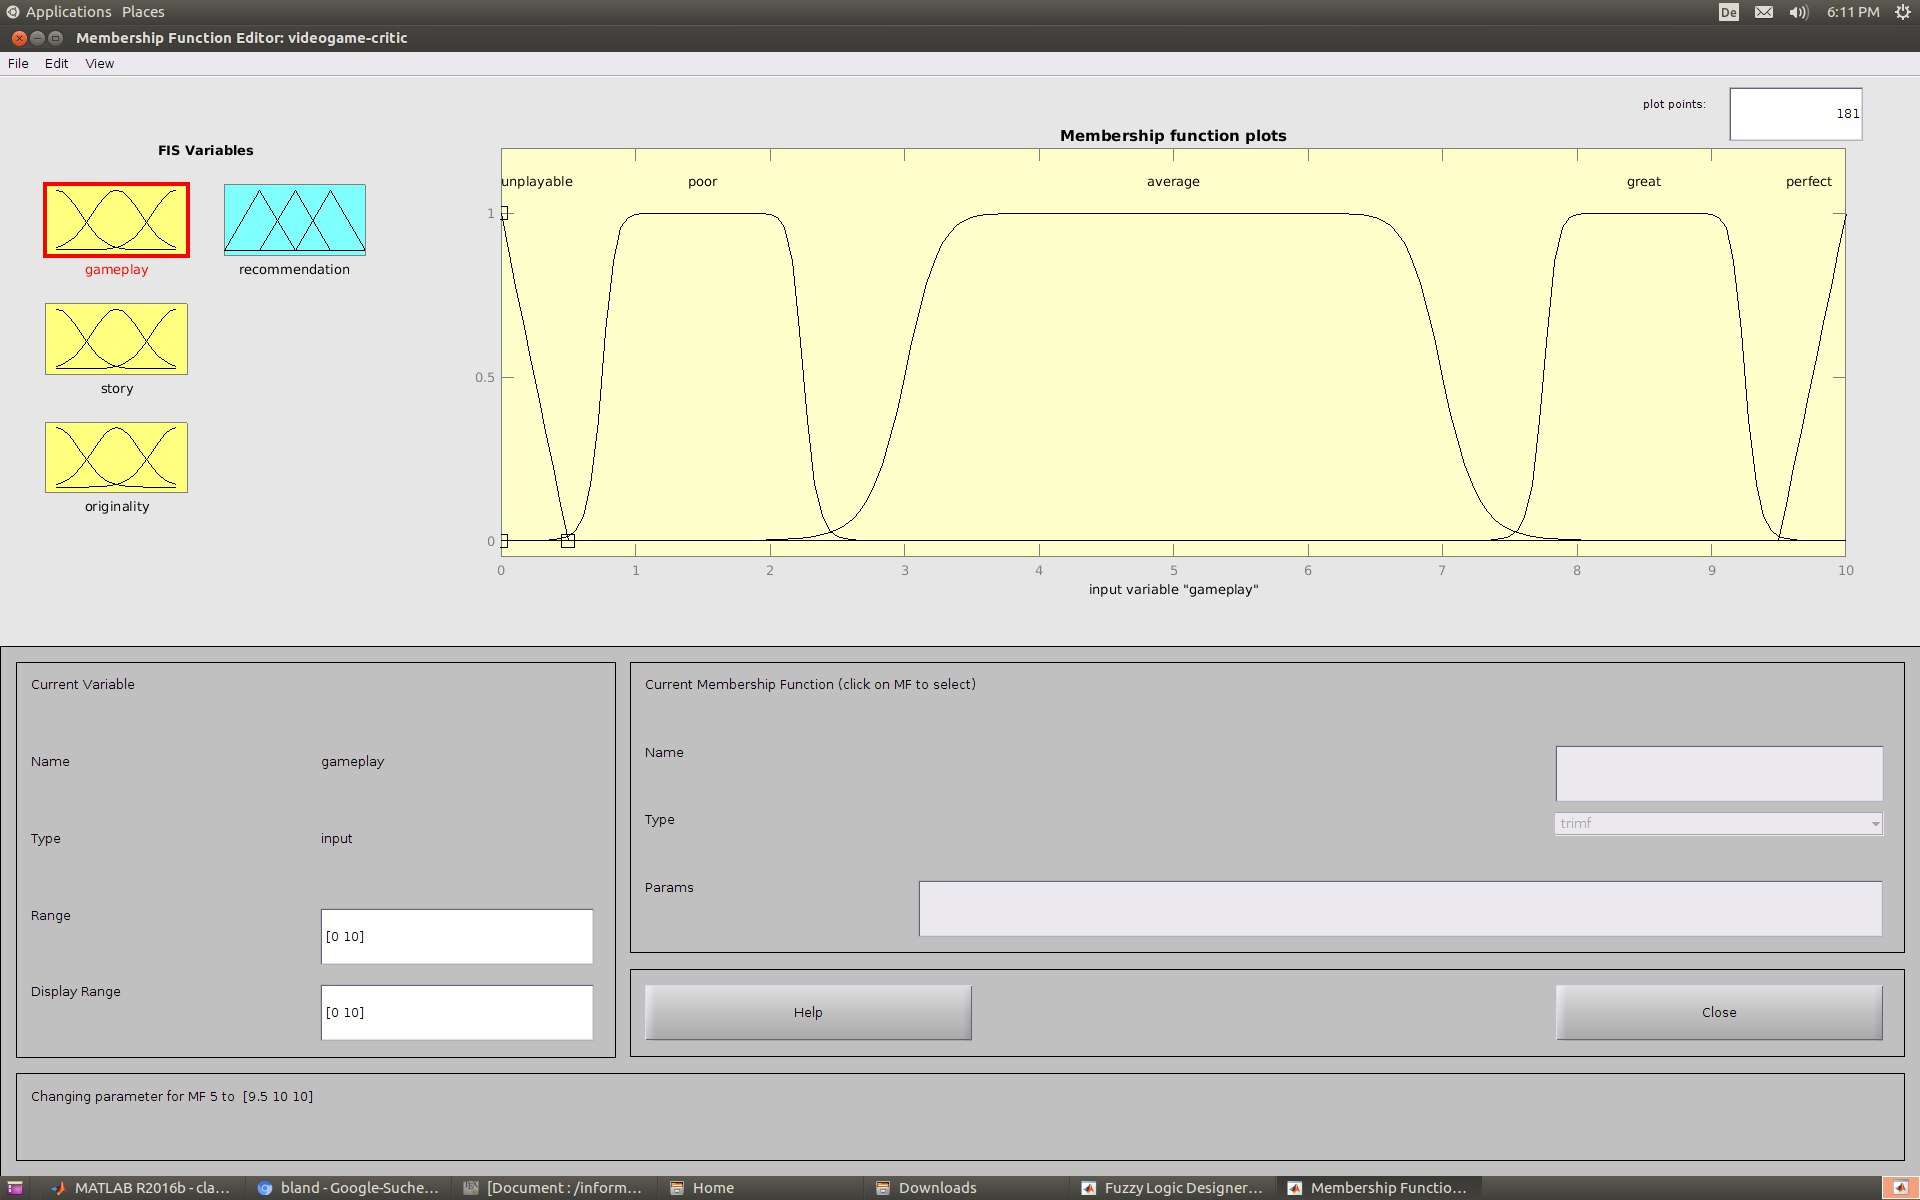
\includegraphics[scale=0.15]{vg-mf-gameplay.jpg}
\end{figure}

But even though this critic focuses on gameplay, he isn't completely oblivious to the other two categories. If a game is incredibly original or has atrocious story, he won't ignore these facts in his rating. \\
His outlook on stories is kind of boring, with two identical plateaus on both sides.

\begin{figure}[ht]
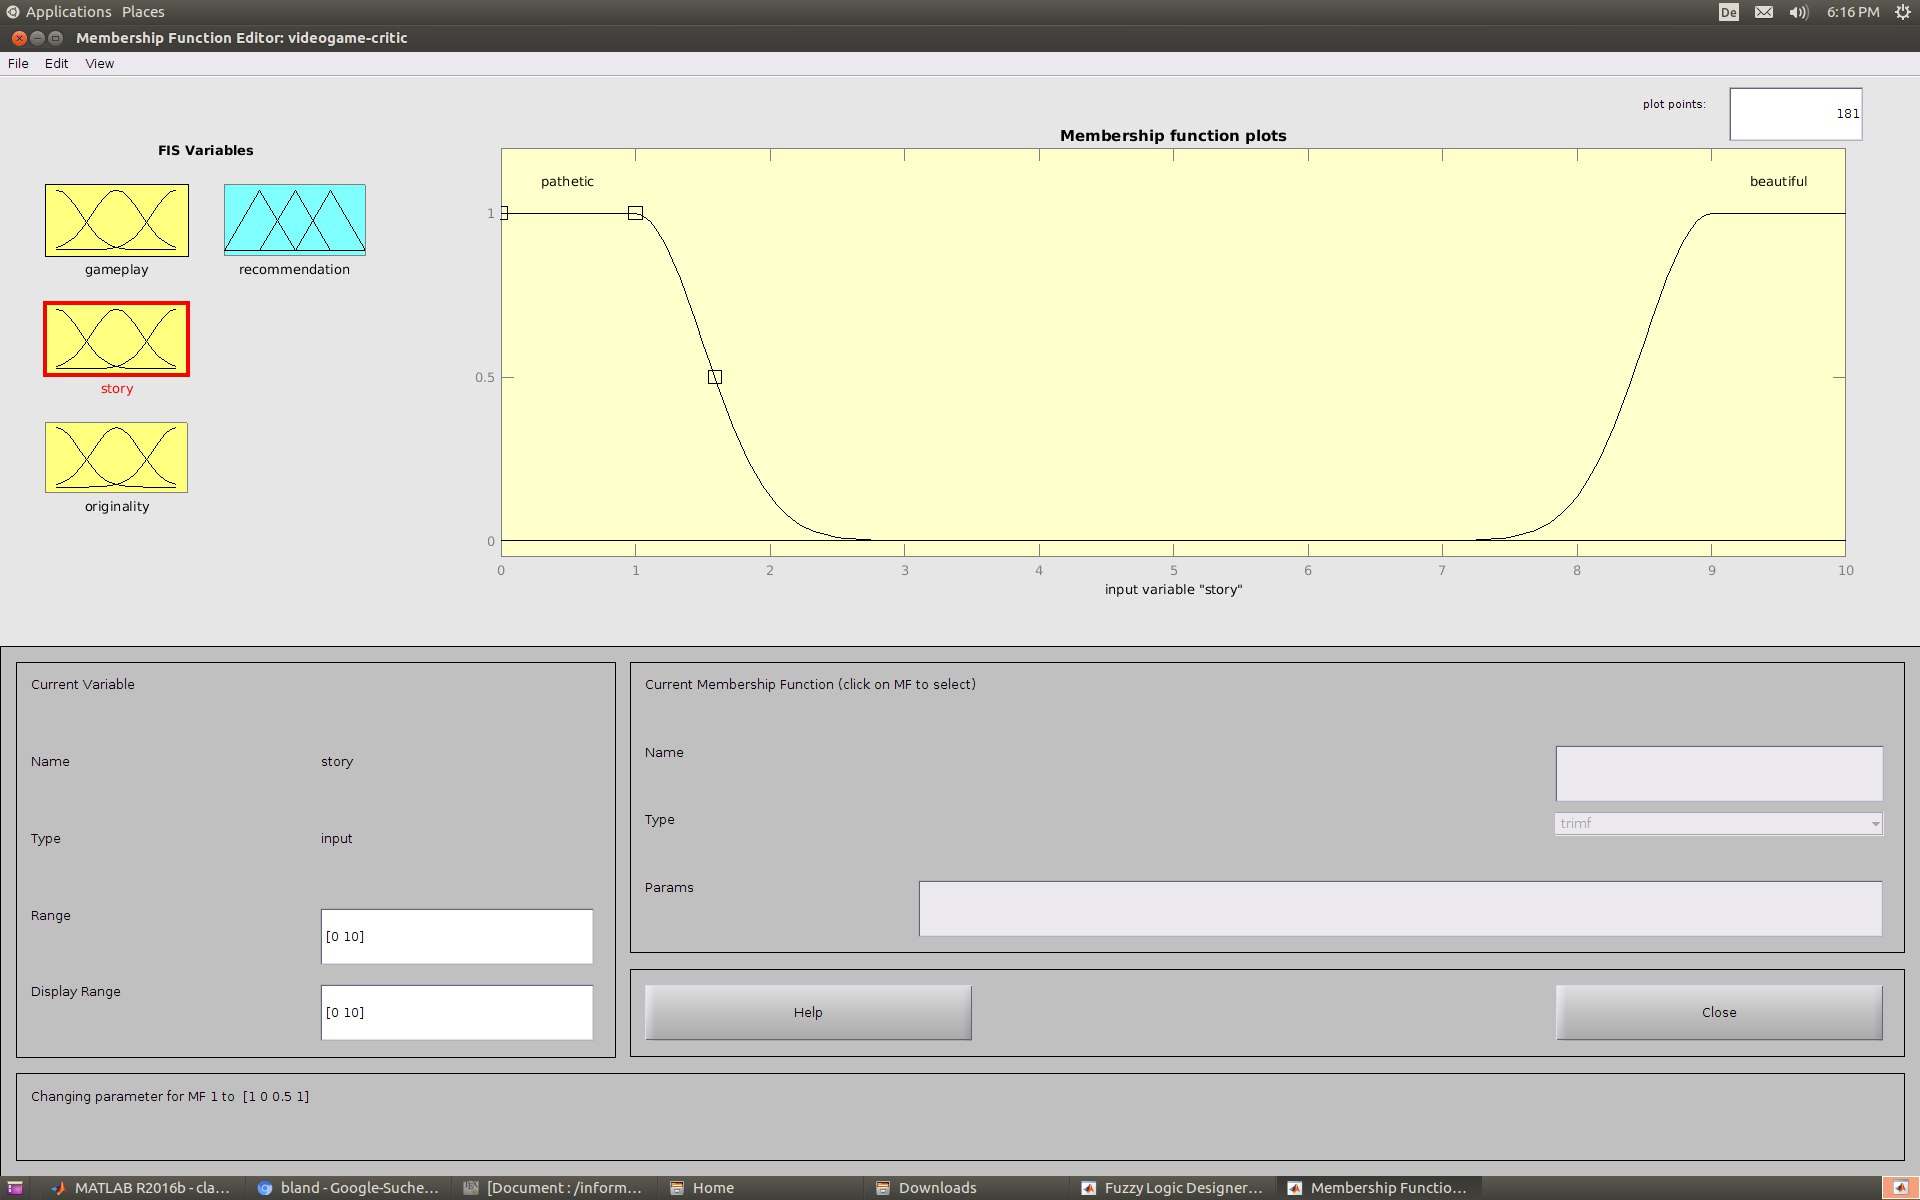
\includegraphics[scale=0.15]{vg-mf-story.jpg}
\end{figure}

\newpage

On the other hand, his view on originality is a bit more unique: If a game completly copied a previous title, it will be very obvious and result in a bad rating. But since videogames are a very iterative medium, he will forgive games that are just very similar to other games, as long as they at least introduce a few new mechanics as well. Naturally, an increased amount of unique mechanics will gradually increase the originality of a title.

\begin{figure}[ht]
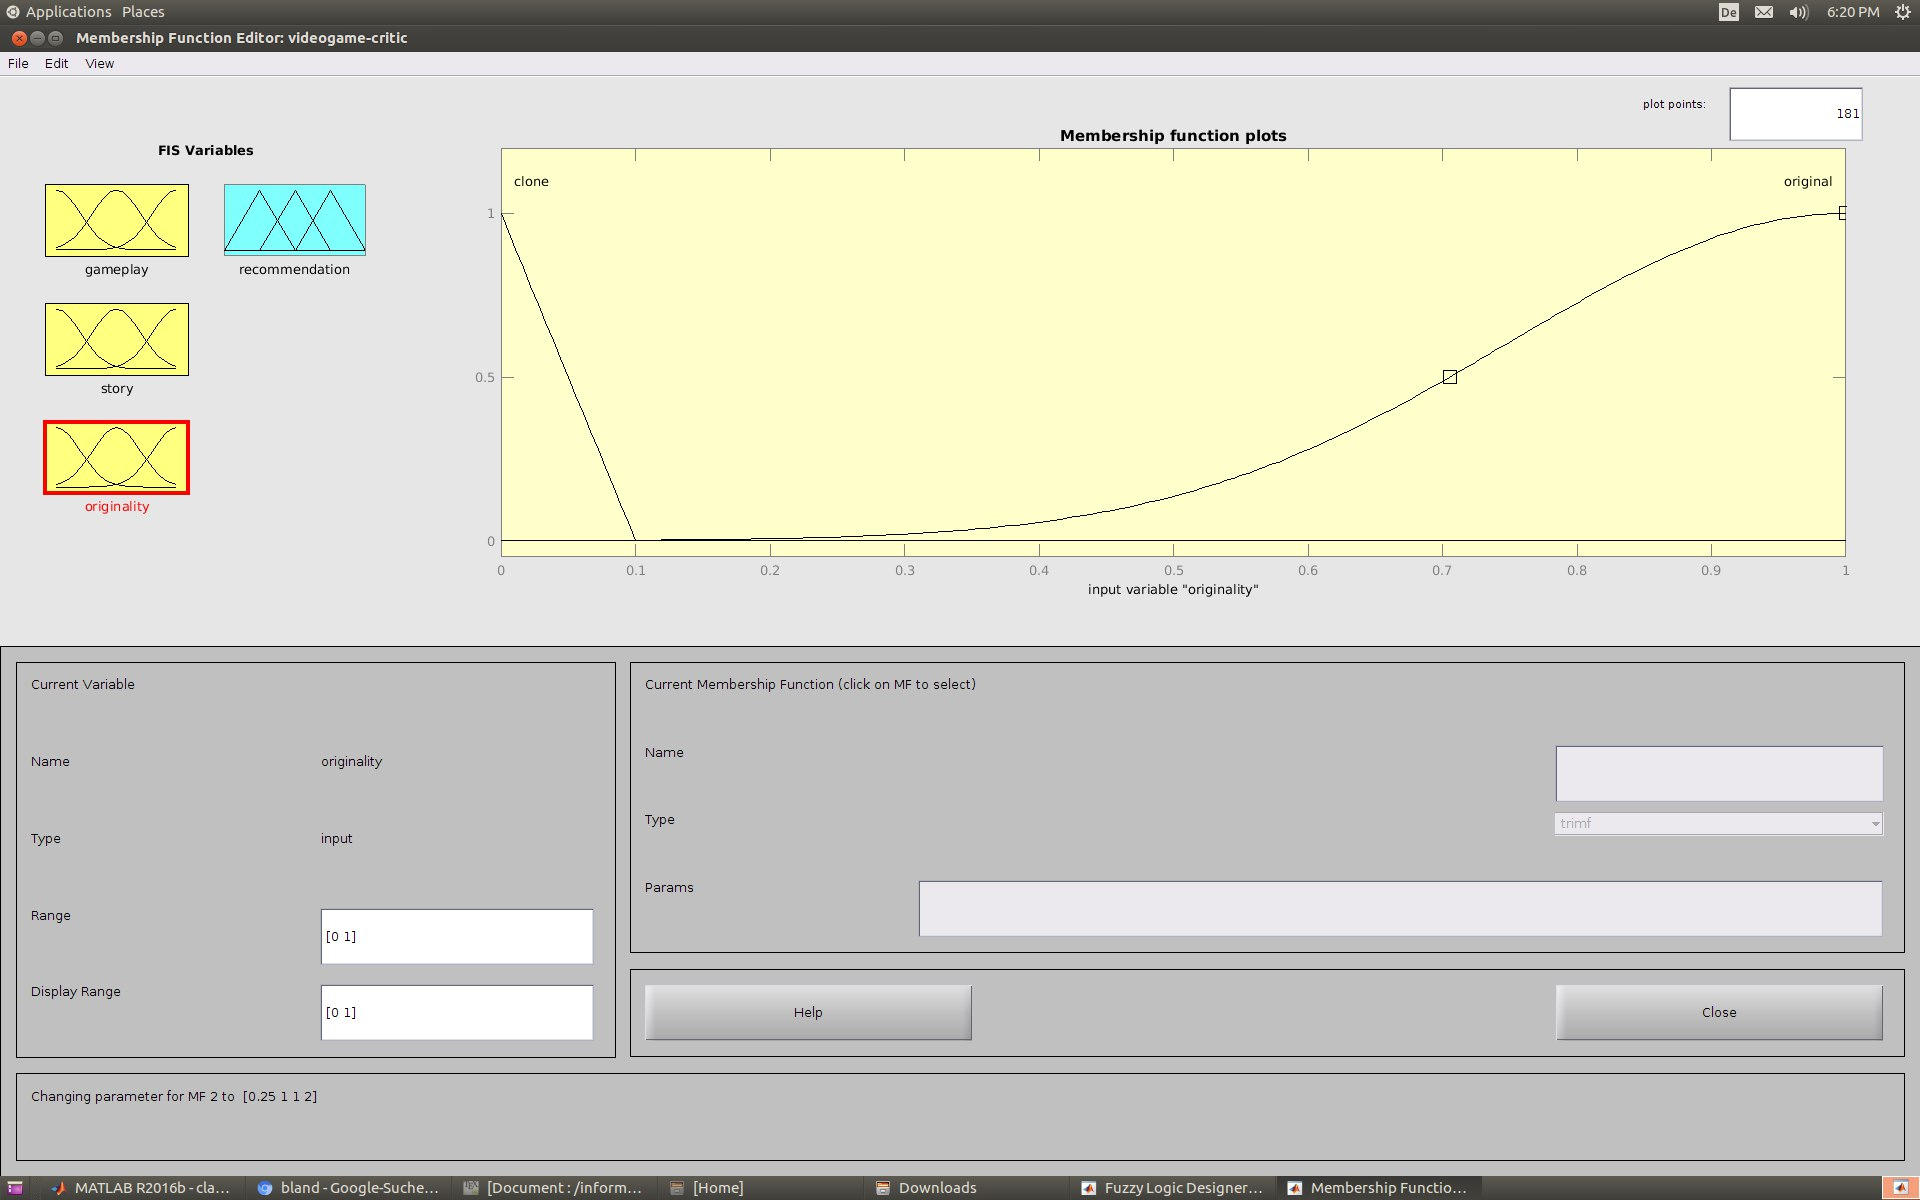
\includegraphics[scale=0.15]{vg-mf-originality.jpg}
\end{figure}

When it comes to rules, \textit{gameplay} is obviously the driving force among all input variables. An \textit{unplayable} game is not worth most people's time while a game with \textit{perfect} gameplay can probably even be enjoyed by people, who aren't the biggest fans of the given genre. \\
\textit{Story} and \textit{originality} do have potential to slighty shift the overall rating on their own. And if both of them happen to be exceptionally extreme in the same direction, they can even counteract an extreme stance of \textit{gameplay}.

\begin{figure}[ht]
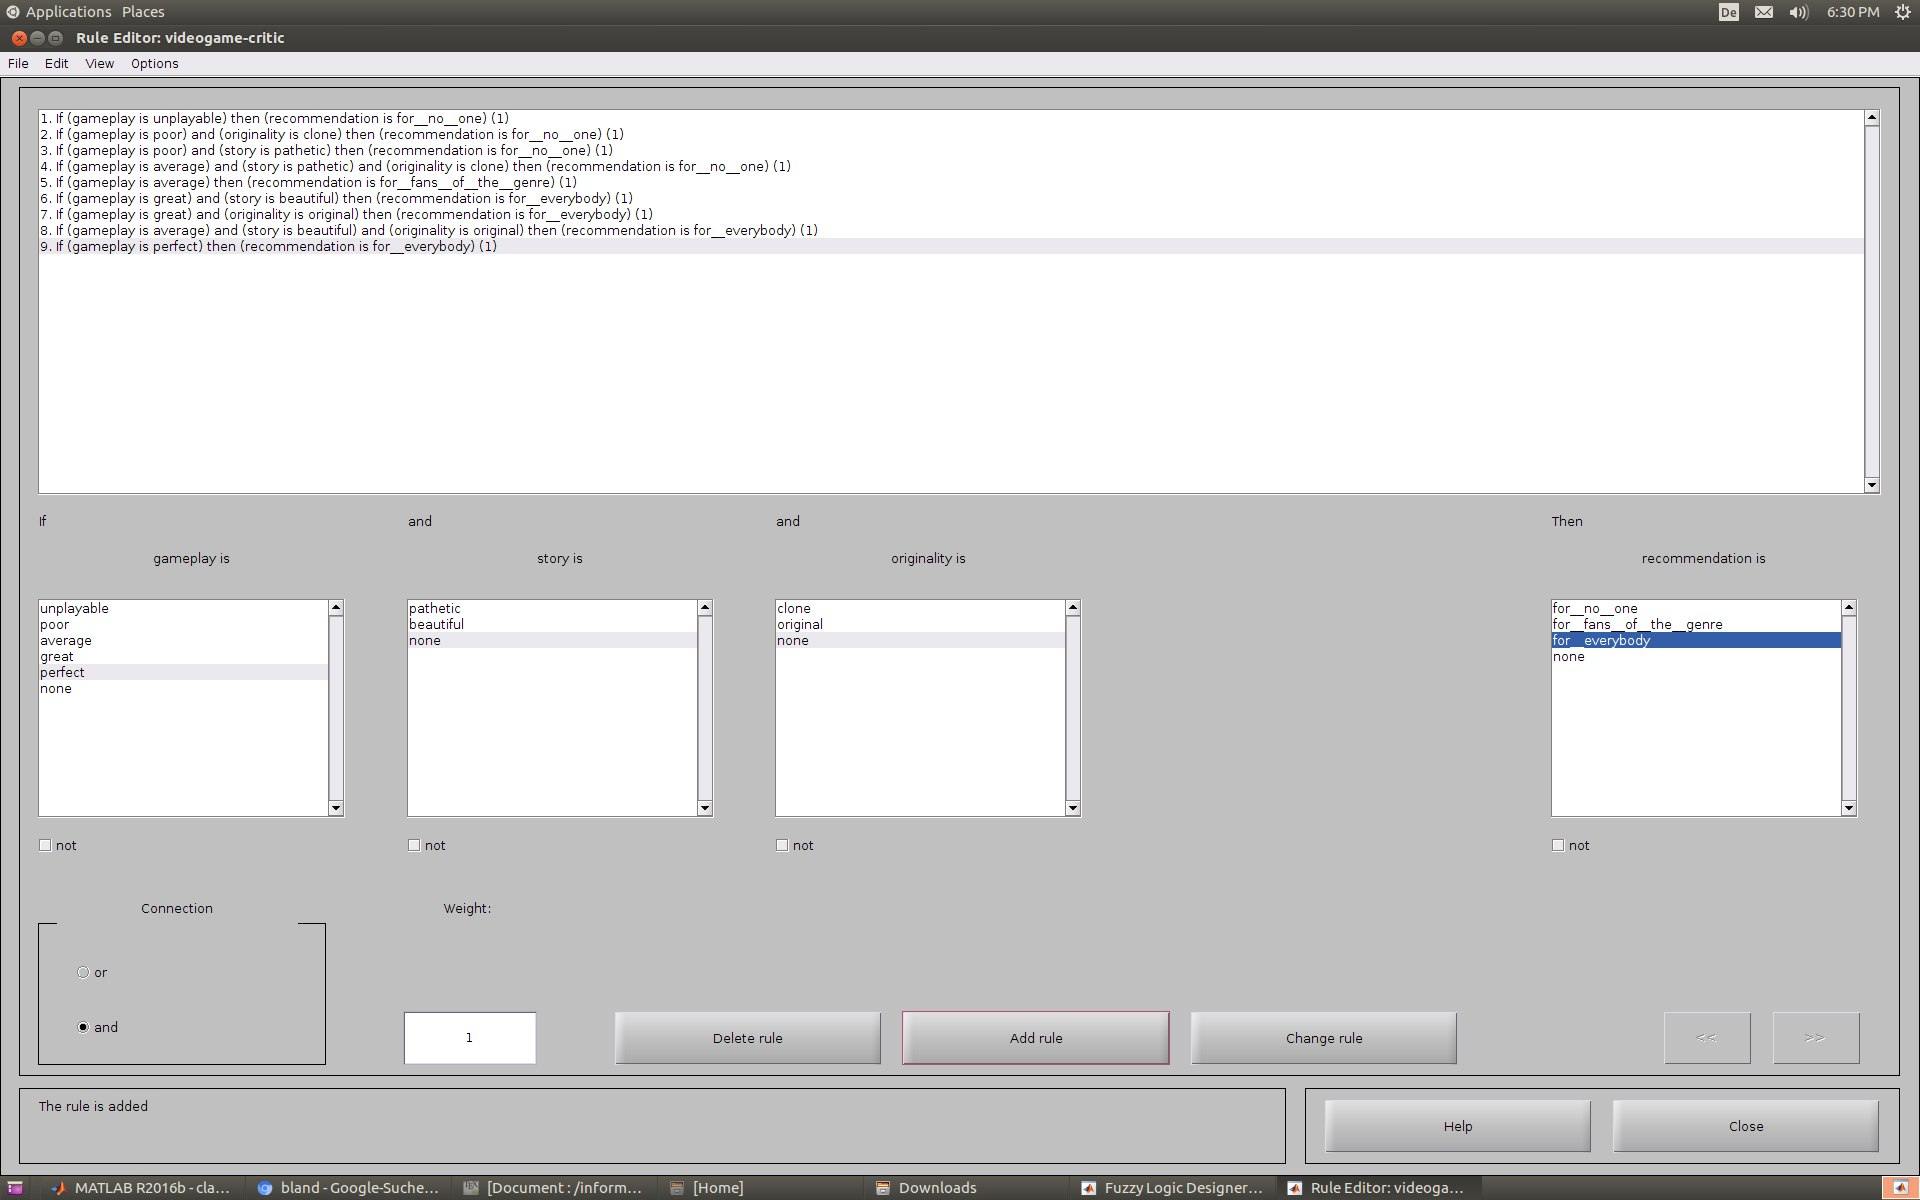
\includegraphics[scale=0.15]{vg-rules.jpg}
\end{figure}

\newpage

With the membership functions and rules in mind, the resulting visualizations seem to be quite intuitive:

\begin{figure}[ht]
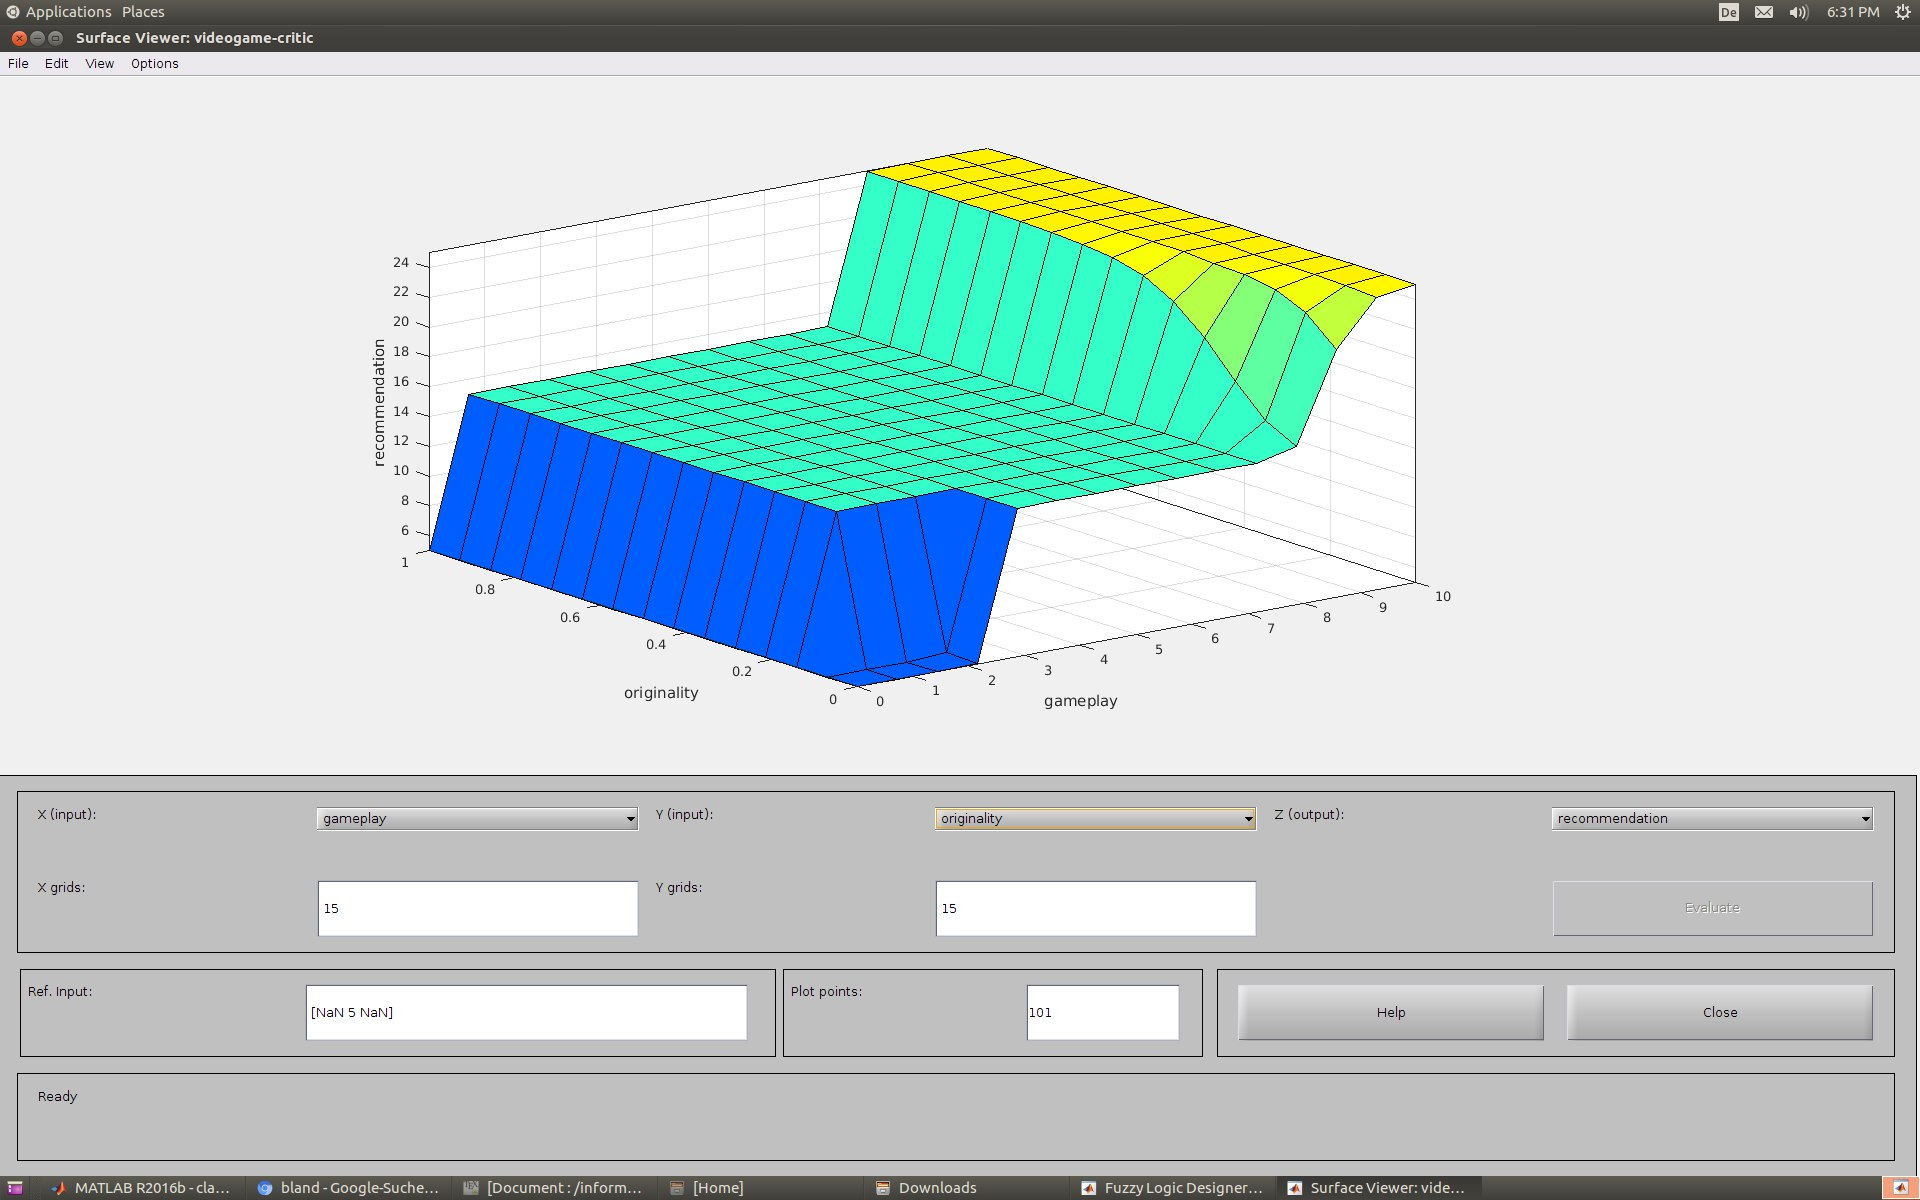
\includegraphics[scale=0.12]{vg-surface-g-o.jpg}
\end{figure}

An \textit{unplayable} game stays at 0 no matter how original, but as soon as the game becomes at least \textit{poor}, the originality gets the power to increase the rating to 50\%. The huge amount of flat surface on this graph is an indicator of how little the originality actually does for the rating, as long as the game in question isn't in the lower end of originality.

\begin{figure}[ht]
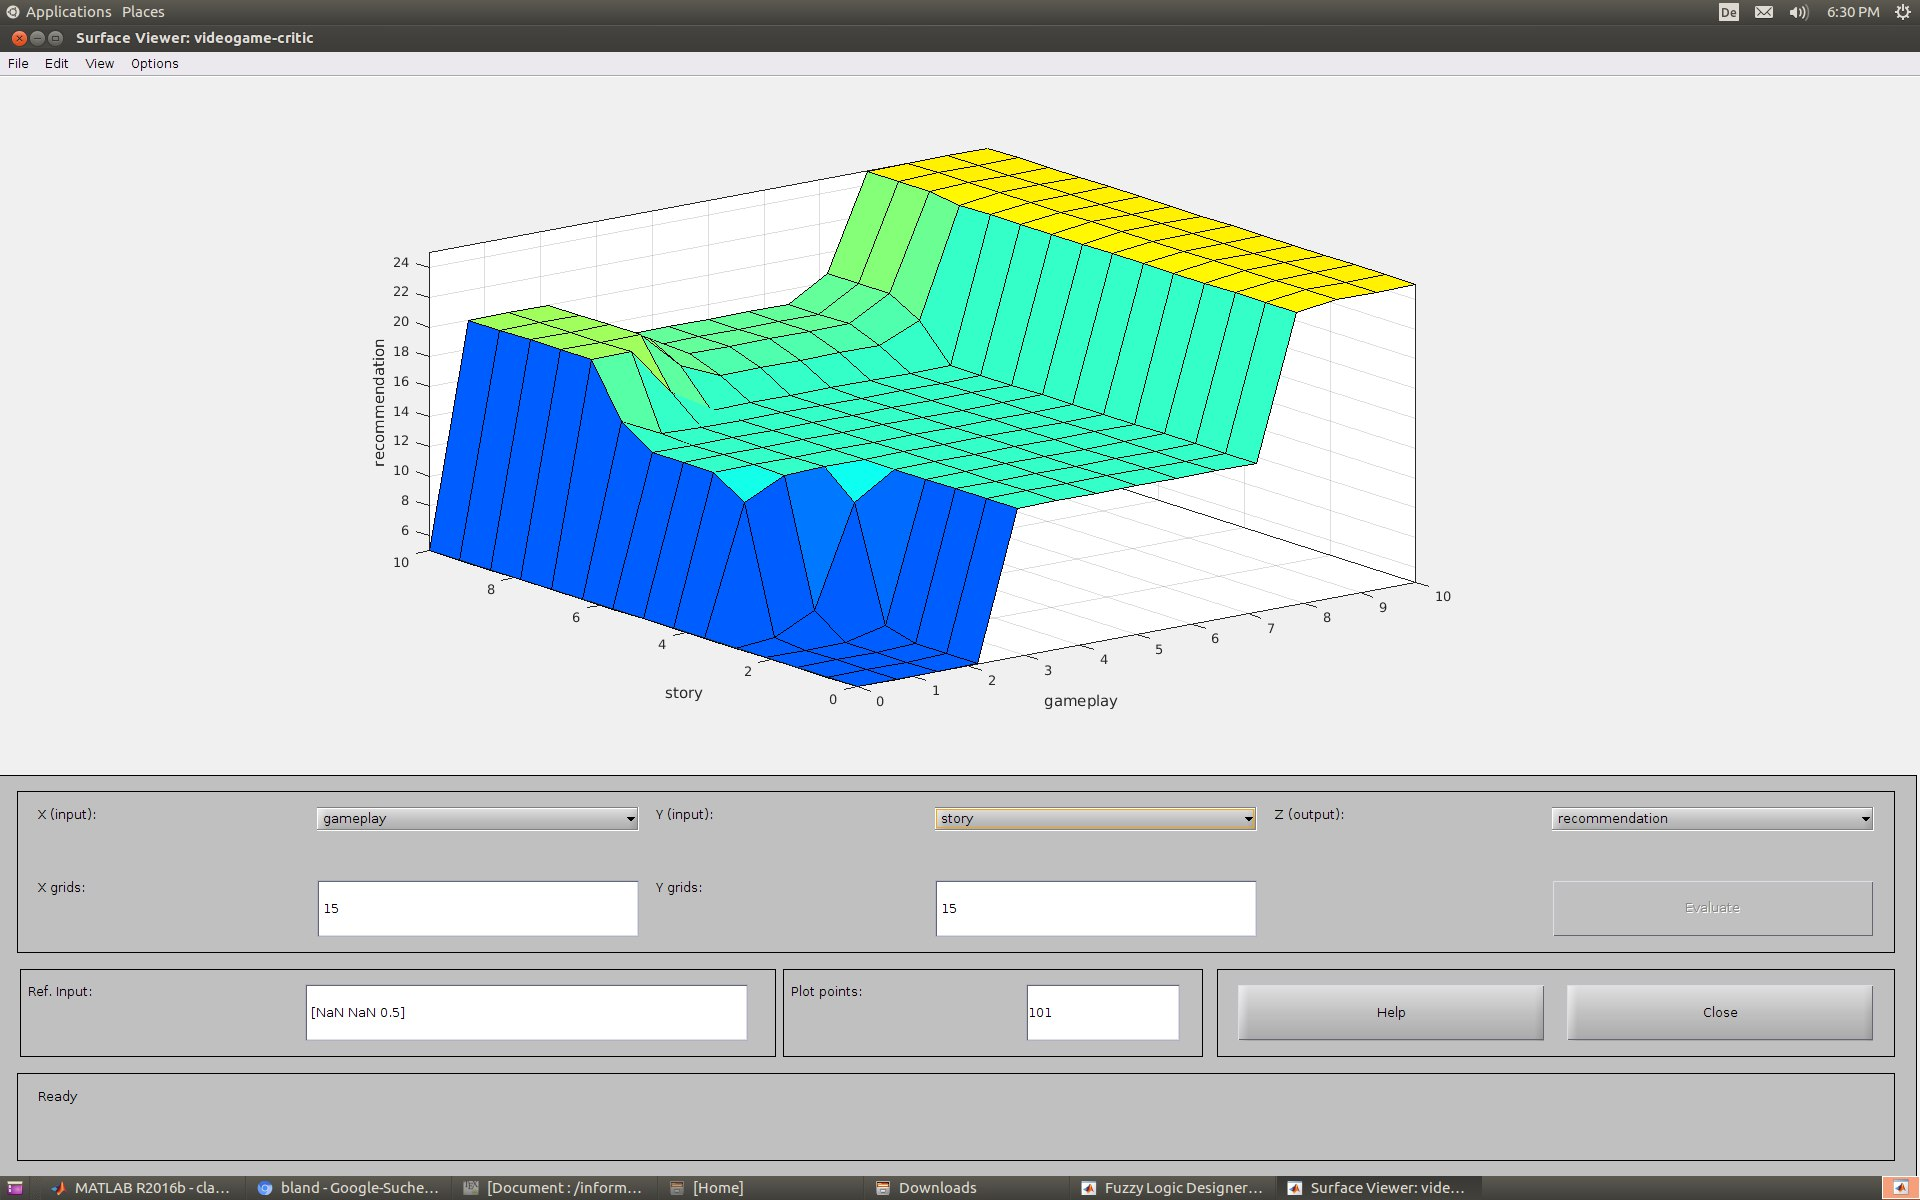
\includegraphics[scale=0.12]{vg-surface-g-s.jpg}
\end{figure}

\textit{Gameplay} and \textit{story} have a more interesting relationship, because \textit{story} doesn't have as much of a steep lower end as originality's \textit{clone} function does. This results in \textit{story} bringing quite a high level of rating without getting past \textit{poor} gameplay. However, gameplay still has the upper hand here and can even bring the rating to a maximum level while keeping \textit{story} at a level of 0.\\ This surface also holds the only major error of the model: At maximum \textit{story}, the overall rating goes back down around \textit{gameplay} level of 2 before going back up at around 6.5, which makes no sense for any critic and especially not for the one I modeled, because gameplay is supposed to be the driving force here.

\newpage

\begin{figure}[ht]
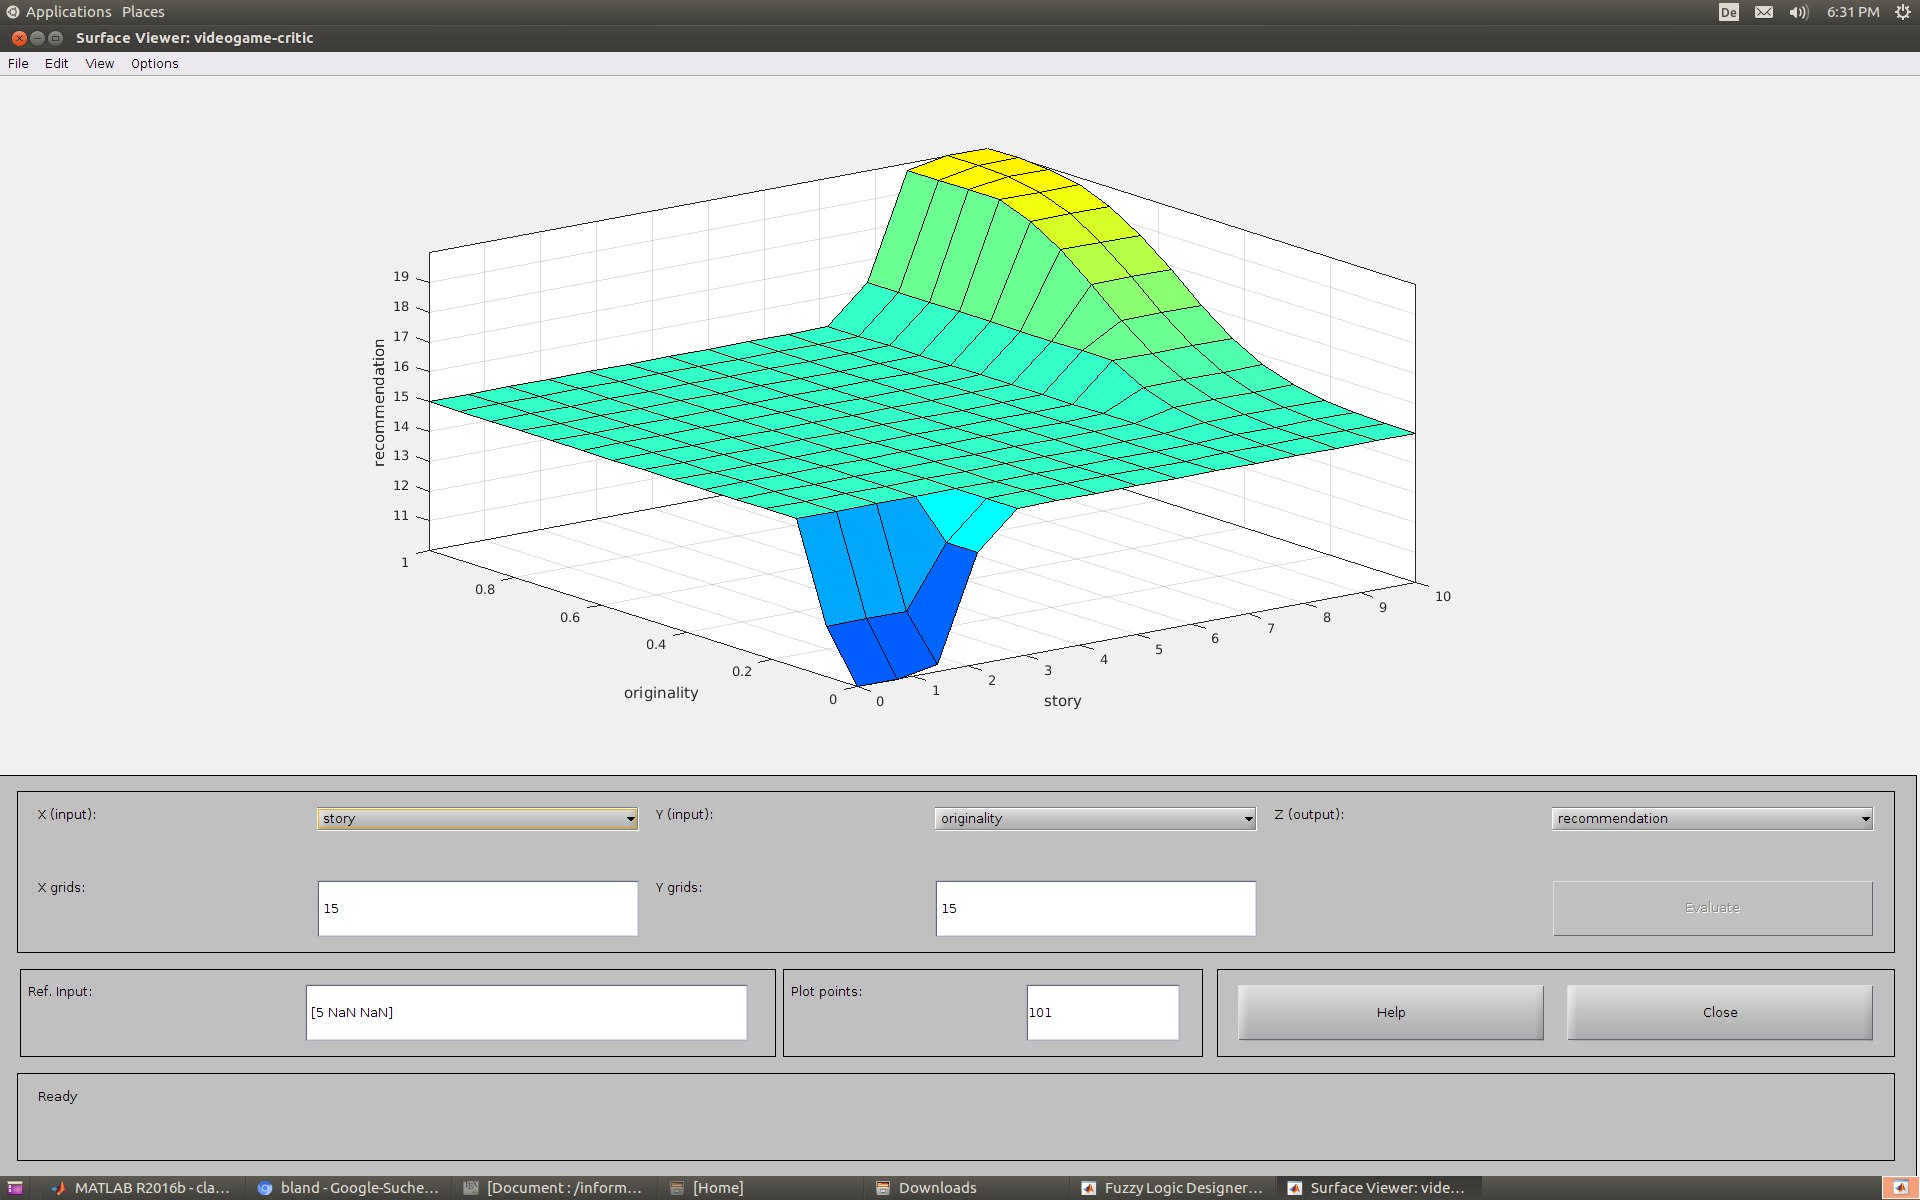
\includegraphics[scale=0.15]{vg-surface-s-o.jpg}
\end{figure}

Finally, we have the relationship of \textit{story} and \textit{originality}. This graph has the most amount of flat surface, which lays on 50\% of the maximum rating. This is also quite intuative, since these two variables only have any impact, if both of them are extremes in the same direction, as explained in the rules above. We can also distinctly see the increase that comes from \textit{originality} due to its unique membership functions.

\end{document}
